\documentclass[border=3pt,tikz]{standalone}
\usepackage{amsmath}
\usetikzlibrary{arrows}
\usetikzlibrary{positioning}
\usetikzlibrary{calc}
\usetikzlibrary{arrows.meta}
\usetikzlibrary{decorations.pathreplacing}
\begin{document}
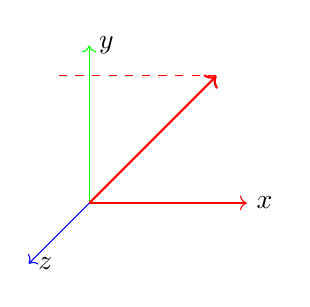
\begin{tikzpicture}
    \draw [red,->](0,0) -- (xyz cs:x=2) node[right, black] {$x$};
    \draw [green,->](0,0) -- (xyz cs:y=2) node[right, black] {$y$};
    \draw [blue,->](0,0) -- (xyz cs:z=2) node[right, black] {$z$};
  
    \draw [red, thick, ->] (0, 0) -- (xyz cs:x=2, y=2, z=1);
    \draw [red, dashed] (xyz cs:x=2, y=2, z=1) -- (xyz cs:x=0, y=2, z=1);
  \end{tikzpicture}
\end{document}